\section{Arquitetura}
\label{sec:architecture}

A arquitetura proposta foi concebida como um sistema de segurança multicamadas para Modelos de Linguagem de Grande Escala (LLMs), estruturado com o objetivo de detectar, mitigar e bloquear ameaças semânticas e estruturais ao longo de todo o ciclo de processamento dos prompts. Essa organização modular distribui responsabilidades entre componentes especializados, permitindo robustez, escalabilidade e transparência no tratamento de riscos associados à interação com LLMs.

A Figura~\ref{fig:architecture_diagram} apresenta uma visão geral da arquitetura, destacando o fluxo de informações entre os módulos e os pontos de verificação de segurança aplicados em cada etapa.

\begin{figure}[ht]
    \centering
    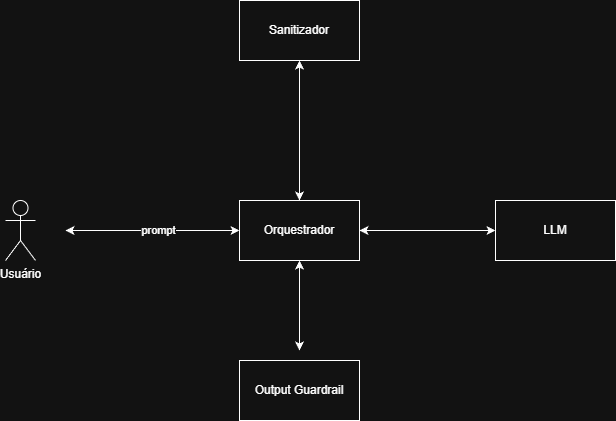
\includegraphics[width=0.48\textwidth]{sections/images/prompt_security_diagram.png}
    \caption{Arquitetura geral do sistema de segurança proposto para LLMs.}
    \label{fig:architecture_diagram}
\end{figure}

\subsection{Componentes Principais}

A arquitetura é composta por quatro módulos centrais:

\begin{enumerate}
    \item \textbf{Sanitizer};
    \item \textbf{Input Guardrail};
    \item \textbf{Bias and Output Guardrail};
    \item \textbf{Orchestrator Service}.
\end{enumerate}

Cada módulo atua de forma complementar, compondo um pipeline de análise capaz de interceptar ameaças explícitas, implícitas e semânticas.

\subsection{Sanitizer}

O \textit{Sanitizer} constitui a primeira linha de defesa. Ele realiza o pré-processamento estrutural dos prompts, assegurando que o conteúdo enviado para as etapas seguintes esteja em formato consistente e livre de artefatos maliciosos.

Suas funções principais incluem:

\begin{itemize}
    \item remoção de caracteres invisíveis e não padronizados;
    \item normalização e limpeza de formatos Unicode;
    \item detecção e neutralização de padrões de evasão e ofuscação;
    \item preservação do conteúdo semântico sempre que possível.
\end{itemize}

Ao padronizar a entrada, o módulo reduz a superfície de ataque e estabelece uma base confiável para as verificações subsequentes.

\subsection{Input Guardrail}

A segunda camada, o \textit{Input Guardrail}, efetua verificações sintáticas e semânticas sobre o texto sanitizado. Seu papel é identificar riscos explícitos antes que o prompt seja encaminhado ao LLM.

Entre suas funções, destacam-se:

\begin{itemize}
    \item identificação de tentativas de \textit{prompt injection};
    \item detecção de padrões de \textit{jailbreak};
    \item classificação de intenções maliciosas;
    \item detecção de informações pessoais identificáveis (PII);
    \item bloqueio imediato de entradas consideradas perigosas.
\end{itemize}

O módulo retorna uma resposta estruturada em caso de violação, garantindo que o LLM nunca receba um prompt inseguro.

\subsection{Bias and Output Guardrail}

A terceira camada é responsável por verificar tanto a entrada quanto a resposta gerada pelo LLM. Esse módulo combina regras sintáticas e classificações semânticas para detectar riscos mais complexos.

As funcionalidades incluem:

\begin{itemize}
    \item detecção de vieses linguísticos em categorias como gênero, raça, idade, corpo, orientação ou classe social;
    \item identificação de alucinações (\textit{hallucinations}) e inconsistências factuais;
    \item bloqueio de conteúdo proibido ou antiético;
    \item detecção de possíveis violações de PII após a geração da resposta.
\end{itemize}

A atuação pós-geração é essencial para impedir que o modelo devolva ao usuário conteúdo inadequado ou incorreto.

\subsection{Orchestrator Service}

O \textit{Orchestrator} coordena todo o fluxo entre os módulos, garantindo que cada etapa seja executada no momento adequado e que todas as verificações sejam cumpridas.

Entre suas responsabilidades, destacam-se:

\begin{itemize}
    \item encaminhar o prompt sanitizado para os módulos apropriados;
    \item decidir se o prompt deve ser processado pelo LLM com base nas verificações anteriores;
    \item avaliar a resposta gerada e aplicar verificações finais;
    \item compor o retorno ao usuário de forma padronizada, incluindo campos como \texttt{blocked}, \texttt{risk\_category}, \texttt{sanitized} e \texttt{llm\_response}.
\end{itemize}

Esse módulo abstrai a complexidade interna da arquitetura e garante interoperabilidade e auditabilidade.

\subsection{Fluxo Operacional}

O fluxo operacional completo pode ser descrito em seis etapas:

\begin{enumerate}
    \item O usuário envia um prompt bruto.
    \item O \textit{Sanitizer} limpa e normaliza a entrada.
    \item O \textit{Input Guardrail} verifica se há riscos explícitos.
    \item Caso aprovado, o prompt segue para o LLM.
    \item A resposta gerada é analisada pelo \textit{Bias and Output Guardrail}.
    \item O \textit{Orchestrator} compila o resultado final e retorna ao usuário.
\end{enumerate}

Esse fluxo garante que tanto a entrada quanto a saída sejam avaliadas, configurando uma defesa integrada de ponta a ponta.

\subsection{Justificativa Arquitetural}

A adoção de uma arquitetura multicamadas fundamenta-se na diversidade de ameaças enfrentadas por sistemas baseados em LLMs. Variações nos tipos de ataque, na origem da interferência e na natureza dos riscos exigem um sistema capaz de operar em múltiplos níveis analíticos.

A arquitetura proposta:

\begin{itemize}
    \item evita dependência de um único módulo para detecção de riscos;
    \item possibilita evolução modular com inclusão de novos mecanismos;
    \item assegura interpretabilidade e rastreabilidade das decisões;
    \item promove conformidade ética e redução de vieses prejudiciais.
\end{itemize}

Assim, a arquitetura estabelece uma base robusta para mecanismos avançados de segurança, sustentando os experimentos e análises discutidos na Seção~\ref{sec:resultados_finais}.


